\documentclass{article}
\usepackage[utf8]{inputenc}
\usepackage{blindtext}
\usepackage{graphicx}
\usepackage[pass]{geometry}
\usepackage[backend=bibtex, maxbibnames=99]{biblatex}
\usepackage{parskip}
\usepackage[spanish]{babel}
\usepackage{csquotes}
\usepackage{amssymb}
\usepackage{amsmath}
\usepackage{mathtools}
\usepackage{amsthm}
\usepackage{float}
\usepackage{multicol}


\addbibresource{bibliography.bib} %Imports bibliography file

\begin{document}

\newgeometry{bottom=2.5cm, left=2.1cm,right=2.1cm,top=2.5cm}

\title{Regresión Avanzada \\ Proyecto Final}

\author{Mario~Becerra Contreras \\ Edgar~López}

\date{Otoño 2017}


\maketitle

%!TEX root = ../GLM_Becerra_Lopez.tex

\section{Introducción}
\label{sec:intro}

Intro chidilla.

%!TEX root = ../GLM_Becerra_Lopez.tex

\section{Datos}
\label{sec:datos}

Antes de pasar al análisis de los datos, hay que mencionar que la ciudad de Nueva York está dividida en 5 distritos (\textit{boroughs}), los cuales a su vez están divididos en 42 vecindarios, los cuales están divididos en 178 códigos postales. Los datos tienen información de venta en 154 códigos postales en todos los vecindarios y, por ende, en todos los distritos.

\subsection{Gráficas univariadas}

La principal variable de interés es el precio en dólares de venta de las casas en Nueva York. En la figura \ref{fig:eda_histograma_precio_venta} se muestra una gráfica de frecuencias absoluta con y sin la transformación logaritmo. Como se puede observar, los precios de venta se asemejan a una distribución exponencial o gamma, pero aplicando la transformación logaritmo, los datos se asemejan a una muestra de una distribución normal, por lo que se usará esta transformación en los modelos posteriores.

\begin{figure}[H]
    \centering
    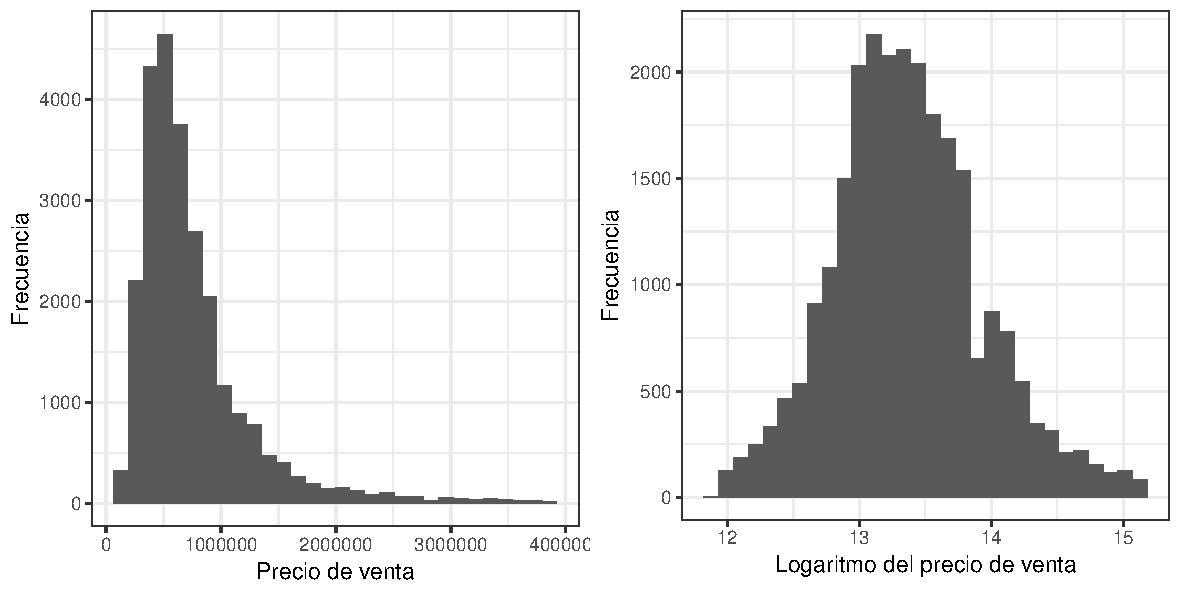
\includegraphics[width=0.9\textwidth]{images/eda_histograma_precio_venta.pdf}
    \caption{Histogramas del precio de venta en escala original y en escala logarítmica}
    \label{fig:eda_histograma_precio_venta}
\end{figure}


Otra de las variables de interés es la superficie total que esta medida en pies cuadrados. La figura \ref{fig:eda_histograma_superficie} muestra las gráficas de frecuencias absolutas para esta variable con y sin transformación logaritmo. De igual manera que el precio de ventas, sería más conveniente usar los datos usando la transformación logaritmo pues muestran un comportamiento semejante a una muestra de una distribución normal.

\begin{figure}[H]
    \centering
    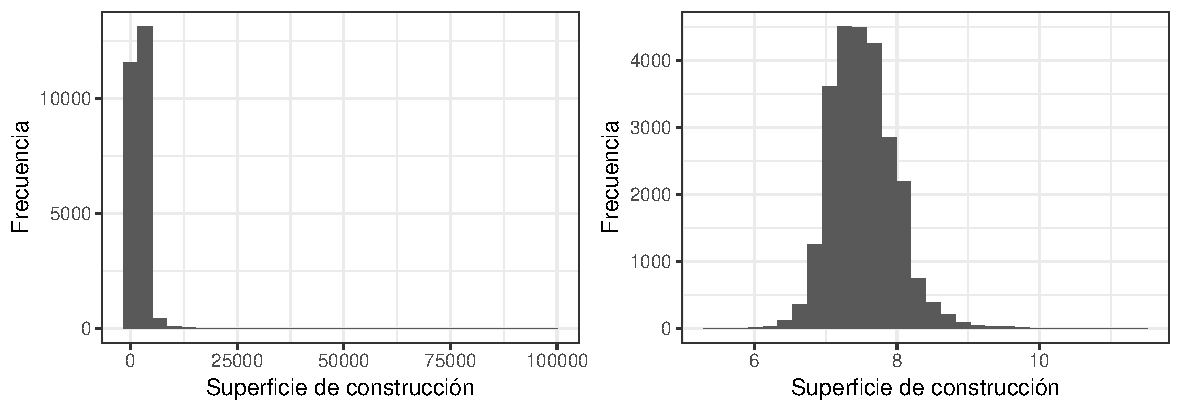
\includegraphics[width=0.9\textwidth]{images/eda_histograma_superficie.pdf}
    \caption{Histogramas de la superficie de construcción en escala original y en escala logarítmica}
    \label{fig:eda_histograma_superficie}
\end{figure}


Finalmente, la variable de superficie del terreno en pies cuadrados se muestra en la figura \ref{fig:eda_histograma_superficie_total_land}. En este caso también sería conveniente usar la transformación logaritmo en los datos pues mejora la distribución muestral y reescala los datos a una escala más pequeña.

\begin{figure}[H]
    \centering
    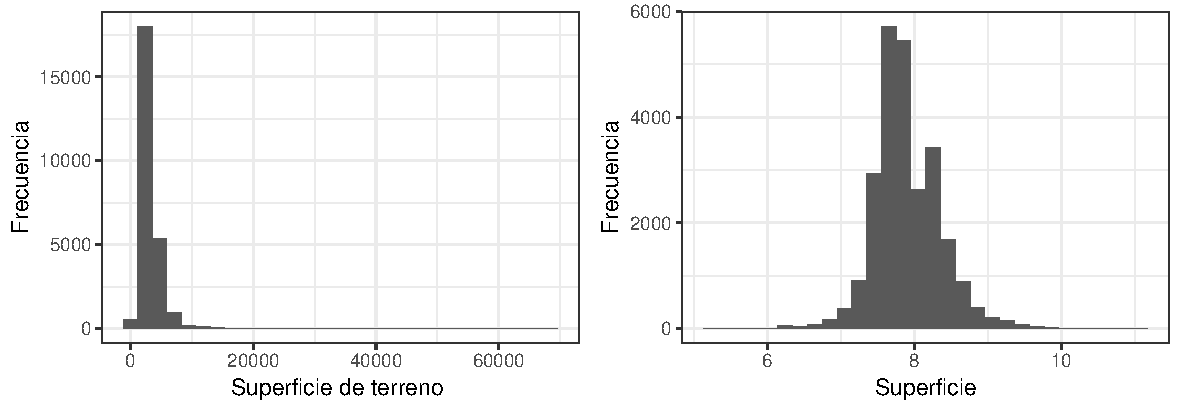
\includegraphics[width=0.9\textwidth]{images/eda_histograma_superficie_total_land.pdf}
    \caption{Histogramas de la superficie del terreno en escala original y en escala logarítmica}
    \label{fig:eda_histograma_superficie_total_land}
\end{figure}






\subsection{Gráficas bivariadas}

Primero se analizará la posible relación entre el precio de venta y la superficie total mediante un diagrama de dispersión. En la figura \ref{fig:eda_dispersion_superficie_vs_precio} se puede ver la gráfica de dispersión de la superficie de construcción contra el precio. Existe una tendencia lineal creciente entre las dos variables, es decir, a mayor superficie total también se tiene un mayor precio de venta. Por lo que la variable de superficie total puede ser usada como variable explicativa en un modelo de regresión.

\begin{figure}[H]
    \centering
    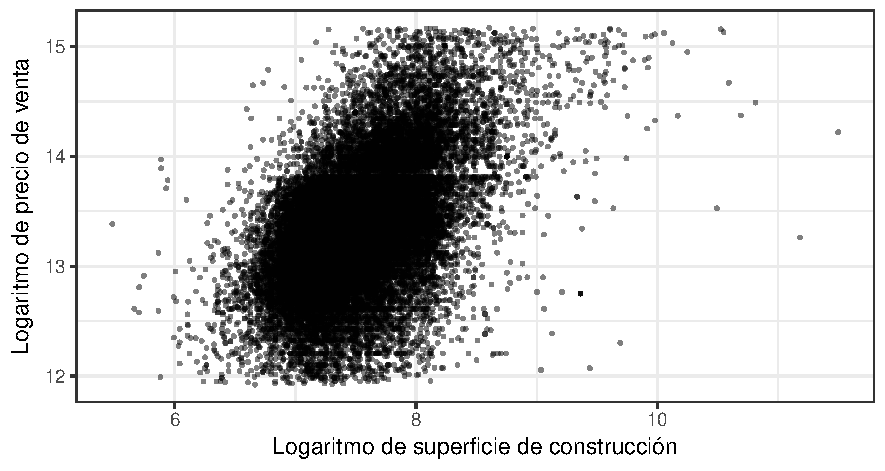
\includegraphics[width=0.7\textwidth]{images/eda_dispersion_superficie_vs_precio.pdf}
    \caption{Gráfica de dispersión de superficie de construcción contra precio}
    \label{fig:eda_dispersion_superficie_vs_precio}
\end{figure}


La relación entre la superficie de terreno y el precio de venta se muestra en el diagrama de dispersión de la figura \ref{fig:eda_dispersion_superficie_total_vs_precio}. Visualmente no existe una relación entre estas dos variables pues no muestra alguna tendencia. En la figura \ref{fig:eda_dispersion_superficie_total_vs_superficie} se muestra la posible relación entre las covariables superficie de construcción y superficie de terreno. Como es de esperarse, estas dos variables están relacionadas pues se puede esbozar una relación creciente, es decir, a mayor superficie total se tiene mayor superficie. Dada esta colinealidad, en un modelo de regresión se debería de usar alguna de estas dos variables pues proporcionan la misma información. En el caso de este trabajo, se seleccionó la variable de superficie de construcción debido a su correlación con el precio.


\begin{figure}[H]
    \centering
    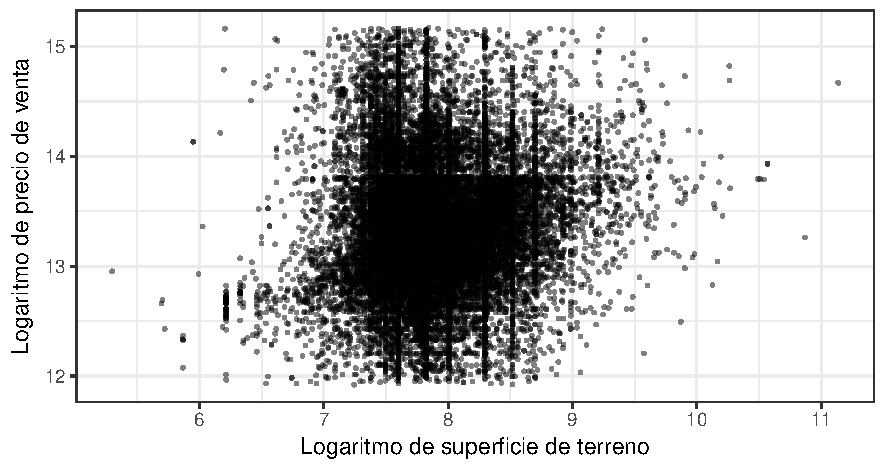
\includegraphics[width=0.7\textwidth]{images/eda_dispersion_superficie_total_vs_precio.pdf}
    \caption{Gráfica de dispersión de superficie de terreno contra precio}
    \label{fig:eda_dispersion_superficie_total_vs_precio}
\end{figure}


\begin{figure}[H]
    \centering
    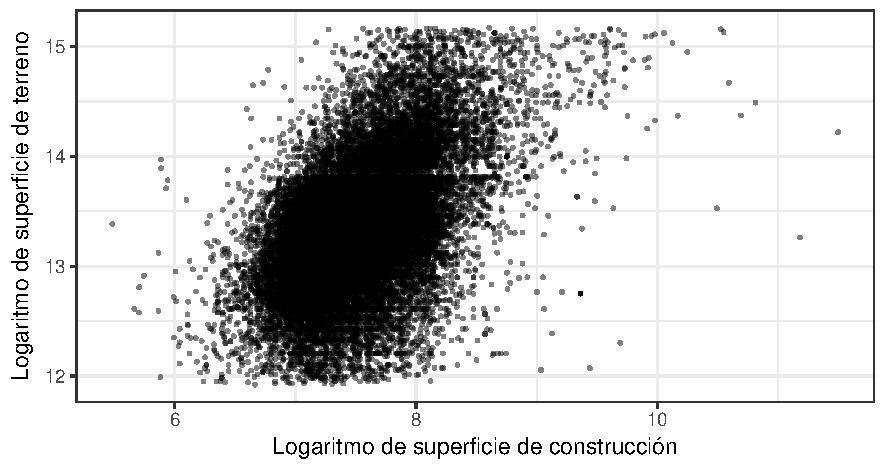
\includegraphics[width=0.7\textwidth]{images/eda_dispersion_superficie_total_vs_superficie.pdf}
    \caption{Gráfica de dispersión de superficie de construcción contra superficie del terreno}
    \label{fig:eda_dispersion_superficie_total_vs_superficie}
\end{figure}


Es de esperar que el precio de venta cambie dependiendo si la casa esta ubicada en cierto distrito (\textit{borough}). Para corroborar esta hipótesis se graficaron los precios en cada uno de los distritos, los cuales se pueden ver en las figuras \ref{fig:eda_histogram_price_borough} y \ref{fig:eda_boxplot_price_borough}. Se puede ver que, en efecto, cambian las distribuciones muestrales dependiendo el distrito en el que se encuentran las casas. También se puede ver que Manhattan muestra una media más alta que el resto de los distritos (línea punteada en figura \ref{fig:eda_boxplot_price_borough}), y también presenta más variación en los precios de venta. El siguiente distrito con una media más alta es Brooklyn con una variación más grande que el resto de los distritos (sin considerar Manhattan). 

\begin{figure}[H]
    \centering
    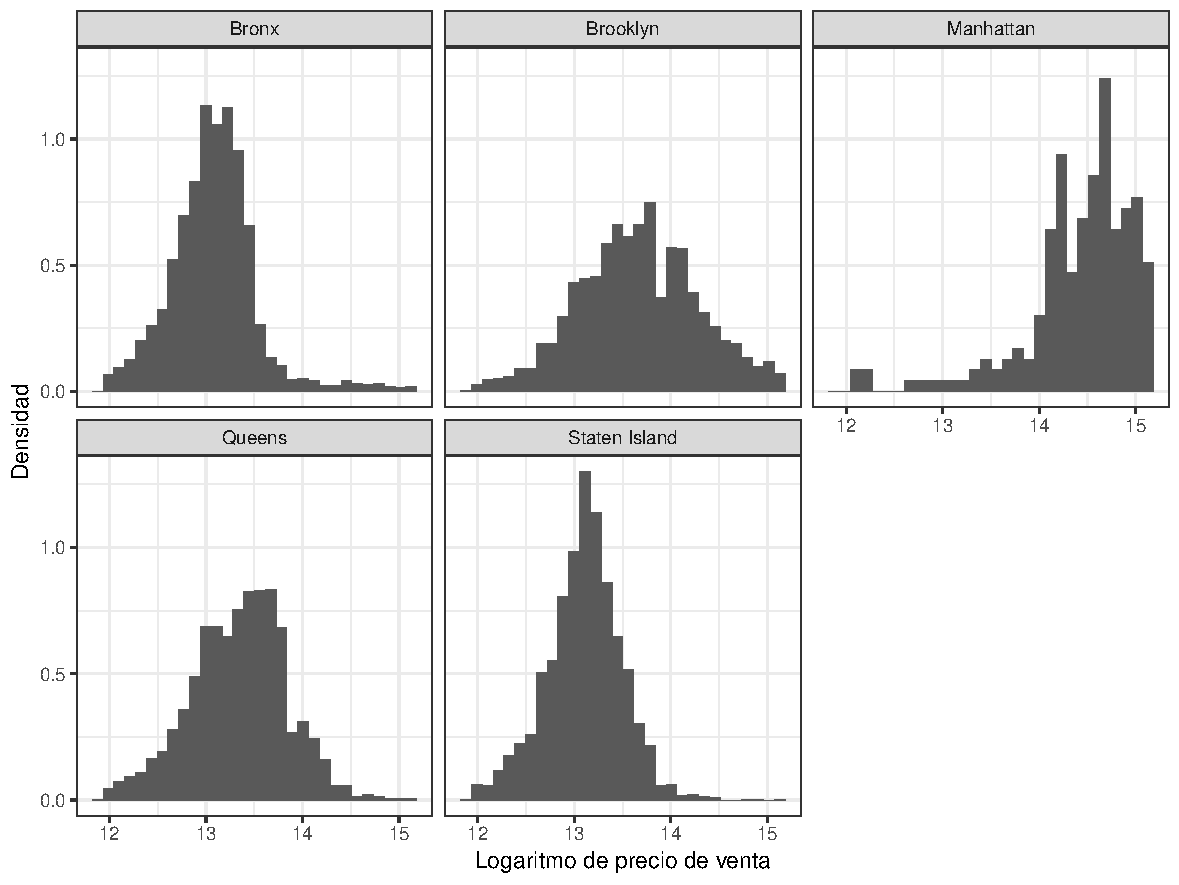
\includegraphics[width=0.7\textwidth]{images/eda_histogram_price_borough.pdf}
    \caption{Histogramas de precio de venta por distrito}
    \label{fig:eda_histogram_price_borough}
\end{figure}


\begin{figure}[H]
    \centering
    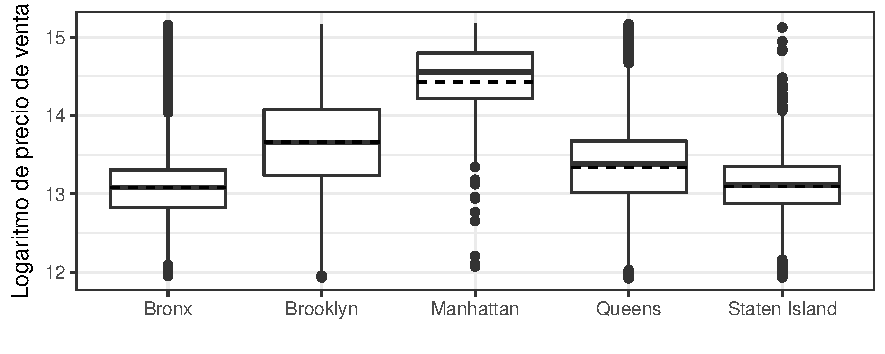
\includegraphics[width=0.7\textwidth]{images/eda_boxplot_price_borough.pdf}
    \caption{Diagrama de caja y brazos de precio de venta por distrito}
    \label{fig:eda_boxplot_price_borough}
\end{figure}

 

Hasta este momento se ha omitido la variable vecindario en el análisis exploratorio. La figura \ref{fig:eda_scatter_by_neighborhood} muestra la dispersión de los datos en cada vecindario. Se puede observar que considerando los vecindarios dentro de cada distrito, en algunos la relación creciente no es tan clara, o incluso llega a verse decreciente, como en el Upper West Side de Manhattan. Hay que tomar en cuenta que el número de observaciones en este vecindario es más pequeño. %Por ejemplo, en el distrito de Queens, los vecindarios Southeast Queens y Rockaways. Sin embargo los datos parecen seguir agrupandose por el tipo de casa que es. Tambien se puede observar que no en todas los vecindarios se encuentran todos los tipos de casas.

El propósito de esta gráfica es mostrar que las relaciones cambian de vecindario a vecindario, por lo que hay que tomar esto en cuenta al momento de hacer los modelos. Aún cuando existe otro nivel geográfico (los códigos postales), no es factible graficar la relación a este nivel pues son demasiados para que se pueda ver en una hoja, sin embargo, se hizo un análisis y también se ve que las relaciones cambian.

\begin{figure}[H]
    \centering
    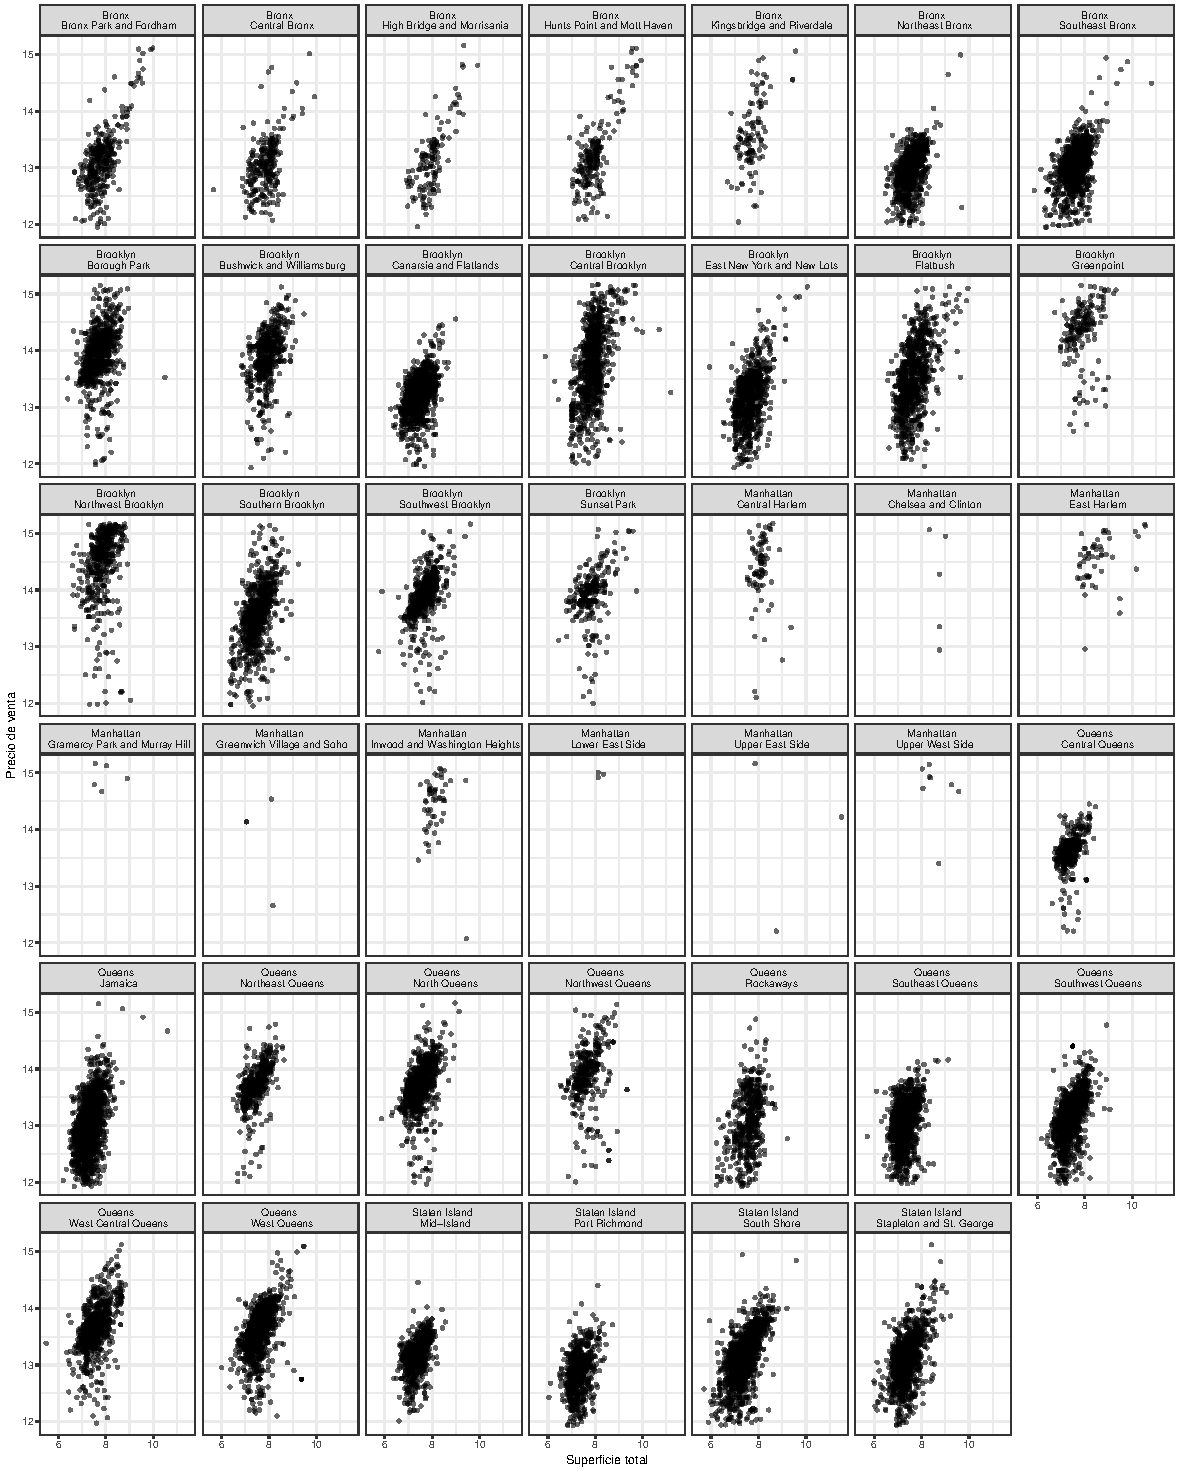
\includegraphics[width=1.03\textwidth]{images/eda_scatter_by_neighborhood.pdf}
    \caption{Diagramas de dispersión del logaritmo del precio contra el logaritmo del tamaño en cada vecindario}
    \label{fig:eda_scatter_by_neighborhood}
\end{figure}



%!TEX root = ../GLM_Becerra_Lopez.tex

\section{Modelos estadísticos}
\label{sec:modelos}

El objetivo es obtener estimaciones del precio de las casas a partir del tamaño en pies cuadrados. Para probar la capacidad predictiva, se dividieron los datos en dos: un conjunto de entrenamiento con el 90\% de los datos, y un conjunto de prueba con el 10\% restante. Para tener información de todos los códigos postales, se hizo un muestreo estratificado, tomando el 90\% de observaciones de cada código postal para el conjunto de entrenamiento. En el conjunto de entrenamiento quedaron $22,769$ observaciones y en el de prueba $2,530$.	

Se ajustaron tres modelos lineales a los datos: un modelo de unidades iguales, un modelo de unidades independientes, y un modelo jerárquico. El modelo de unidades iguales asume que todas las realizaciones provienen de la misma distribución; mientras que el de unidades independientes asume que los precios varían de acuerdo a diferentes sectores (en este caso son los códigos postales); y finalmente, el modelo jerárquico es un compromiso entre ambos modelos que toma fuerza de los demás sectores, esto es particularmente útil cuando hay sectores con pocas observaciones.

\subsection{Modelo de unidades iguales}

El modelo de unidades iguales es simplemente un modelo de regresión lineal con un parámetro fijo para el intercepto y un parámetro fijo para cada uno de los regresores. Sean $y_i$ el logaritmo del precio de la casa $i$ y $x_i$ el logaritmo del número de pies cuadrados en la casa $i$, para $i \in \left\{1, \hdots, n \right\}$, con $n = 22,769$. El modelo de unidades independientes es $y_i \sim \mathrm{N}(\alpha + \beta x_i, \tau_y)$, con distribuciones previas $\alpha \sim \mathrm{N}(0, 0.001)$, $\beta \sim \mathrm{N}(0, 0.001)$ y $\tau_y \sim \mathrm{Ga}(0.001, 0.001)$. %$\alpha \sim \mathrm{N}(\alpha_0, \tau_{\alpha})$, $\beta \sim \mathrm{N}(\beta_0, \tau_{\beta})$ y $\tau_y \sim \mathrm{Ga}(a, b)$

De antemano se tiene conocimiento como para pensar que este modelo no es el más adecuado para los datos, pues se vio en el análisis exploratorio de datos que los precios varían por código postal, por lo que no es muy sensato suponer que no existen relaciones entre las observaciones. De hecho, en la figura \ref{fig:comp_pooling_resids} se puede ver este efecto. Más adelante se ahonda en este resultado.


\subsection{Modelo de unidades independientes}

Este es un modelo de interceptos y pendientes cambiantes de acuerdo al código postal, es decir, es de la forma 

\[
	y_i \sim \mathrm{N}(\alpha_{j[i]} + \beta_{j[i]}x_i, \tau_y),
\]

donde $j[i]$ se refiere al código postal correspondiente a la $i$-ésima observación. Las distribuciones previas son 

\begin{itemize}
	\item $\alpha[j] \sim \mathrm{N}(0, 0.001)$
	\item $\beta[j] \sim \mathrm{N}(0, 0.001)$
	\item $\tau_y \sim \mathrm{Ga}(0.001, 0.001)$
\end{itemize}

para $j = 1, \hdots, J$, con $J = 154$ el número de códigos postales en la ciudad.

\subsection{Modelo multinivel}

En el modelo multinivel o jerárquico, también ajustamos distintos interceptos y pendientes de acuerdo a cada código postal, pero en lugar de considerar cada código postal como una unidad independiente, se le agregaron dos niveles más de hiperparámetros, correspondientes a los vecindarios de la ciudad, y a cada distrito (\textit{borough}). Además, en este modelo no se asume varianza constante en las observaciones, sino que cambian de acuerdo al código postal.

El modelo ajustado fue de la forma $y_i ~ \sim \mathrm{N}(\alpha_{j[i]} + \beta_{j[i]}x_i, \tau_{j[i]})$, donde nuevamente $j[i]$ se refiere al código postal correspondiente a la $i$-ésima observación. Las distribuciones previas son $\alpha_j \sim \mathrm{N} (\mu_{\alpha, k[j]}, \tau_{\alpha, k[j]})$, $\beta_j \sim \mathrm{N} (\mu_{\beta, k[j]}, \tau_{\beta, k[j]})$ y $\tau_{j[i]} \sim \mathrm{Ga}(\alpha_{y, l[k]}, \beta_{y, l[k]})$, donde $k[j]$ se refiere al vecindario correspondiente al $j$-ésimo código postal, y $l[k]$ se refiere al distrito correspondiente al $k$-ésimo vecindario. Las distribuciones previas de estos hiperparámetros son 

 \begin{multicols}{3}
    \begin{itemize}
		\item $\mu_{\alpha, k[j]} \sim \mathrm{N} (\mu_{\alpha, l[k]}, \tau_{\alpha, l[k]})$
		\item $\tau_{\alpha, k[j]} \sim \mathrm{exp} (\lambda_{\alpha, l[k]})$
		\item $\mu_{\beta, k[j]} \sim \mathrm{N} (\mu_{\beta, l[k]}, \tau_{\beta, l[k]})$
		\item $\tau_{\beta, k[j]} \sim \mathrm{exp} (\lambda_{\beta, l[k]})$
		\item $\alpha_{y, l[k]} \sim \mathrm{exp} (\lambda_{\alpha_y, l[k]})$	\item $\beta_{y, l[k]} \sim \mathrm{exp} (\lambda_{\beta_y, l[k]}$
    \end{itemize}
\end{multicols}


Y sus correspondientes hiperparámetros se distribuyen:

\begin{multicols}{3}
	\begin{itemize}

		\item $\mu_{\alpha, l[k]} \sim \mathrm{N}(\mu_{\alpha_0})$	
		\item $\tau_{\alpha, l[k]} \sim \mathrm{exp}(\lambda_{\tau_{\alpha_0}})$	
		\item $\lambda_{\alpha, l[k]} \sim \mathrm{exp}(\lambda_{\lambda_{\alpha_0}})$	
		\item $\mu_{\beta, l[k]} \sim \mathrm{N}(\mu_{\beta_0})$	
		\item $\tau_{\beta, l[k]} \sim \mathrm{exp}(\lambda_{\tau_{\beta_0}})$	
		\item $\lambda_{\beta, l[k]} \sim \mathrm{exp}(\lambda_{\lambda_{\beta_0}})$	
		\item $\lambda_{\alpha_y, l[k]} \sim \mathrm{exp}(\lambda_{\lambda_{\alpha_y}})$	
		\item $\lambda_{\beta_y, l[k]} \sim \mathrm{exp}(\lambda_{\lambda_{\beta_y}})$	

	\end{itemize}
\end{multicols}

Con sus correspondientes distribuciones previas:

\begin{multicols}{3}
	\begin{itemize}
		\item $\mu_{\alpha_0} \sim \mathrm{N}(0, 0.0001)$	
		\item $\lambda_{\tau_{\alpha_0}} \sim \mathrm{exp}(0.01)$	
		\item $\lambda_{\lambda_{\alpha_0}} \sim \mathrm{exp}(0.01)$	
		\item $\mu_{\beta_0} \sim \mathrm{N}(0, 0.0001)$	
		\item $\lambda_{\tau_{\beta_0}} \sim \mathrm{exp}(0.01)$	
		\item $\lambda_{\lambda_{\beta_0}} \sim \mathrm{exp}(0.01)$	
		\item $\lambda_{\lambda_{\alpha_y}} \sim \mathrm{exp}(0.01)$	
		\item $\lambda_{\lambda_{\beta_y}} \sim \mathrm{exp}(0.01)$	
	\end{itemize}
\end{multicols}

%Se tienen en total 758 parámetros.

En la siguiente sección se muestran los resultados de los tres modelos presentados aquí.



%!TEX root = ../GLM_Becerra_Lopez.tex

\section{Resultados}
\label{sec:resultados}

En las figuras \ref{fig:comp_pooling_resids}, \ref{fig:no_pooling_resids} y \ref{fig:three_levels_resids} se muestran para cada uno de los modelos, los residuales en el eje $y$ y en el eje $x$ se muestra el índice de la observación, donde las observaciones están ordenadas de acuerdo a código postal. En el modelo de unidades iguales es evidente un patrón, que viene de la correlación entre las observaciones que existe dentro de cada código postal. En el modelo de unidades independientes los patrones del código postal ya no son tan evidentes como en el modelo de unidades iguales. Lo mismo pasa con el modelo multinivel, ya no hay un patrón evidente.

\begin{figure}[H]
    \centering
    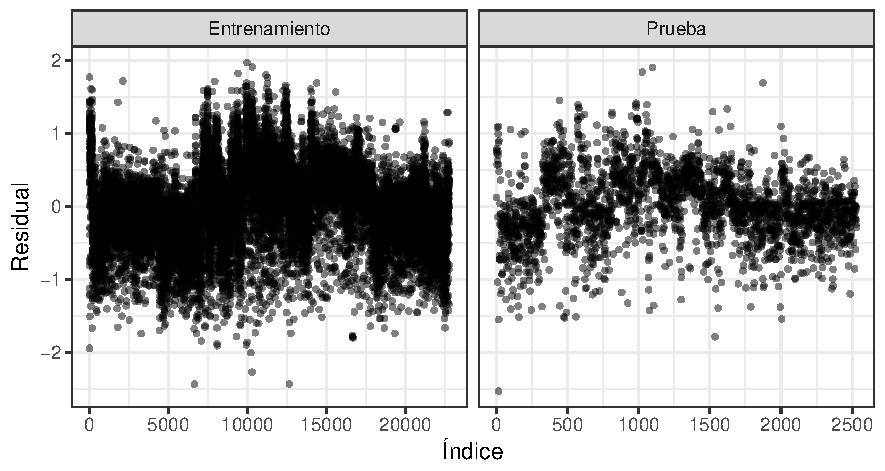
\includegraphics[width=0.7\textwidth]{images/comp_pooling_resids.pdf}
    \caption{Residuales de modelo de unidades iguales}
    \label{fig:comp_pooling_resids}
\end{figure}

\begin{figure}[H]
    \centering
    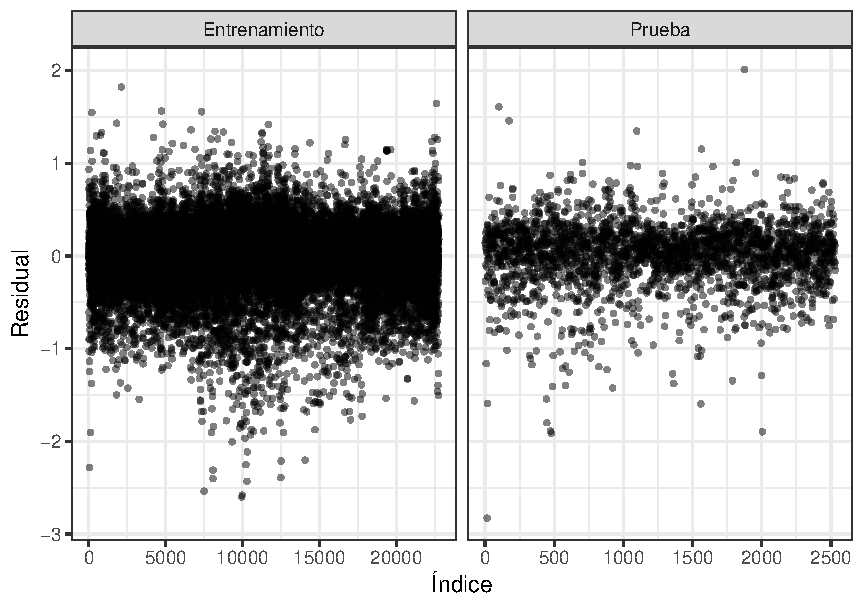
\includegraphics[width=0.7\textwidth]{images/no_pooling_resids.pdf}
    \caption{Residuales de modelo de unidades independientes}
    \label{fig:no_pooling_resids}
\end{figure}

\begin{figure}[H]
    \centering
    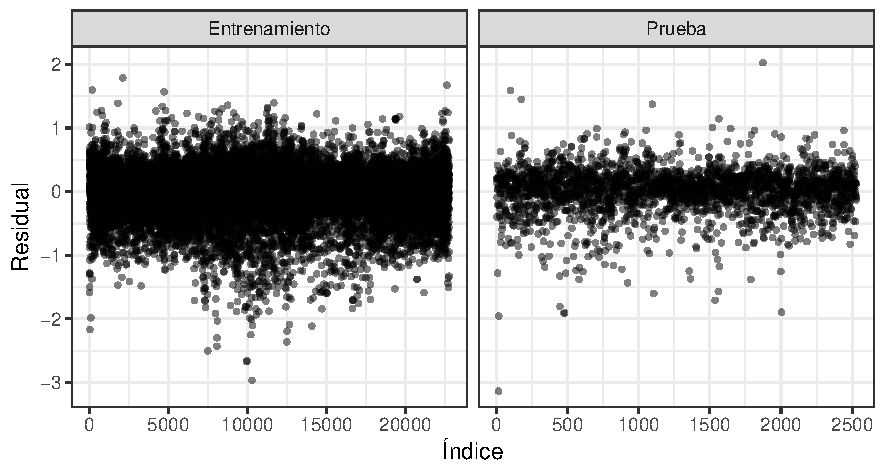
\includegraphics[width=0.7\textwidth]{images/three_levels_resids.pdf}
    \caption{Residuales de modelo multinivel}
    \label{fig:three_levels_resids}
\end{figure}

En las figuras \ref{fig:comp_pooling_obs_vs_pred}, \ref{fig:no_pooling_obs_vs_pred} y \ref{fig:three_levels_obs_vs_pred} se puede ver para cada observación el valor observado contra el valor ajustado de cada modelo. En todos se aprecia una varianza considerablemente grande; y en el modelo de unidades iguales, el modelo tiende a sobreestimar los valores pequeños, mientras que en valores grandes pasa lo contrario. Este efecto persiste, pero en mucho menor medida, en los otros dos modelos.

\begin{figure}[H]
    \centering
    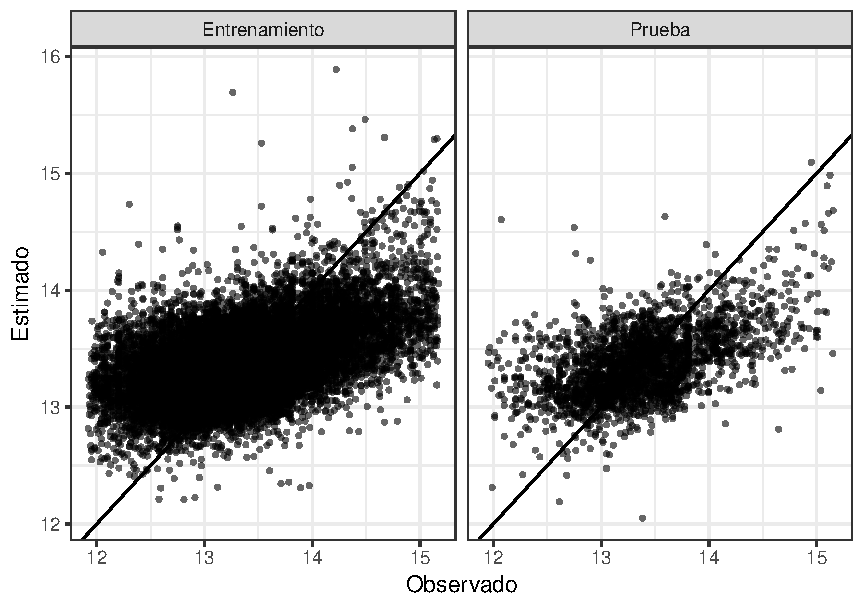
\includegraphics[width=0.7\textwidth]{images/comp_pooling_obs_vs_pred.pdf}
    \caption{Ajustado contra observado en modelo de unidades iguales}
    \label{fig:comp_pooling_obs_vs_pred}
\end{figure}

\begin{figure}[H]
    \centering
    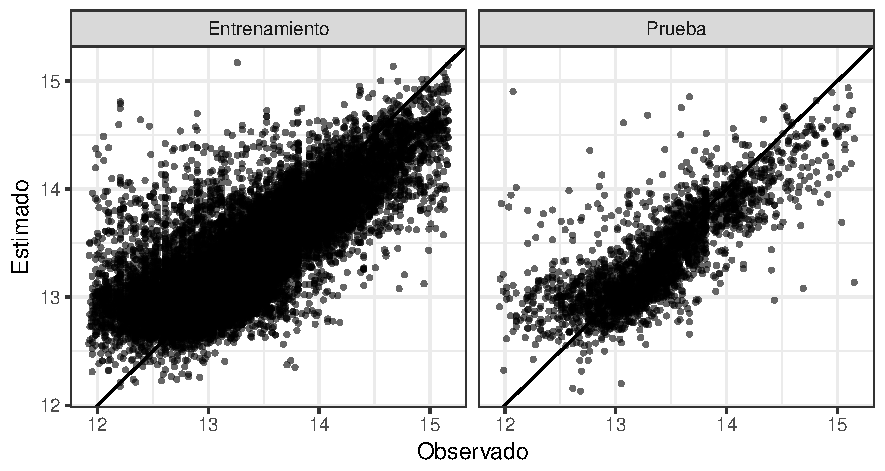
\includegraphics[width=0.7\textwidth]{images/no_pooling_obs_vs_pred.pdf}
    \caption{Valor ajustado contra observado en modelo de unidades independientes}
    \label{fig:no_pooling_obs_vs_pred}
\end{figure}


\begin{figure}[H]
    \centering
    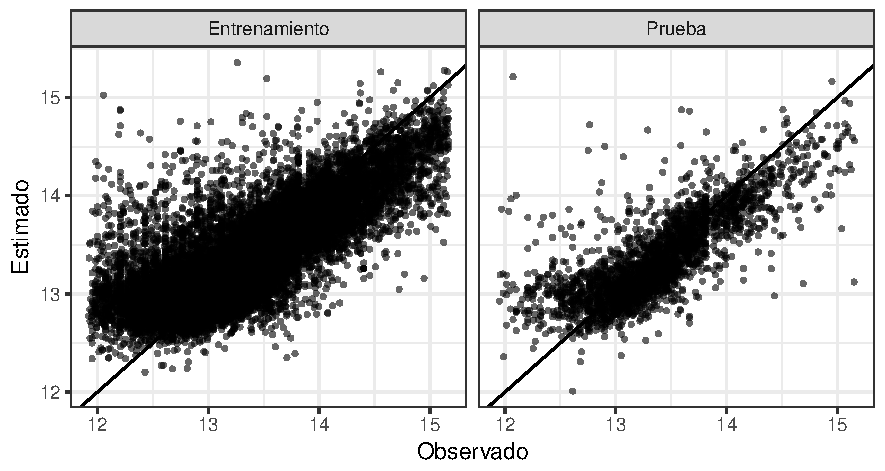
\includegraphics[width=0.7\textwidth]{images/three_levels_obs_vs_pred.pdf}
    \caption{Valor ajustado contra observado en modelo multinivel}
    \label{fig:three_levels_obs_vs_pred}
\end{figure}

En las figuras \ref{fig:no_pooling_param_values} y \ref{fig:three_levels_param_values} se muestran los valores de los parámetros junto con sus intervalos al 95\% de probabilidad del modelo de unidades independientes y del modelo multinivel. En el modelo de unidades independientes hay varios parámetros que tienen una varianza muy grande, y hay incluso algunos códigos postales que tienen un parámetro de pendiente negativo, lo cual intuitivamente no hace mucho sentido, pues eso significaría que a menor tamaño, la casa es más grande; pero recordando el análisis exploratorio, estas estimaciones negativas corresponden a los códigos postales con pocas observaciones en las cuales se podía apreciar una tendencia negativa; pero esto no es nada más que ruido de la muestra pequeña que se tiene. En el modelo multinivel, al tomar fuerzas de los hiperparámetros, no se tienen estimaciones puntuales negativas, y los intervalos de probabilidad son mucho más pequeños; sin embargo, sí se aprecia cambio entre los parámetros; es decir, el modelo está captando las diferencias de precio que existen entre los códigos postales.

\begin{figure}[H]
    \centering
    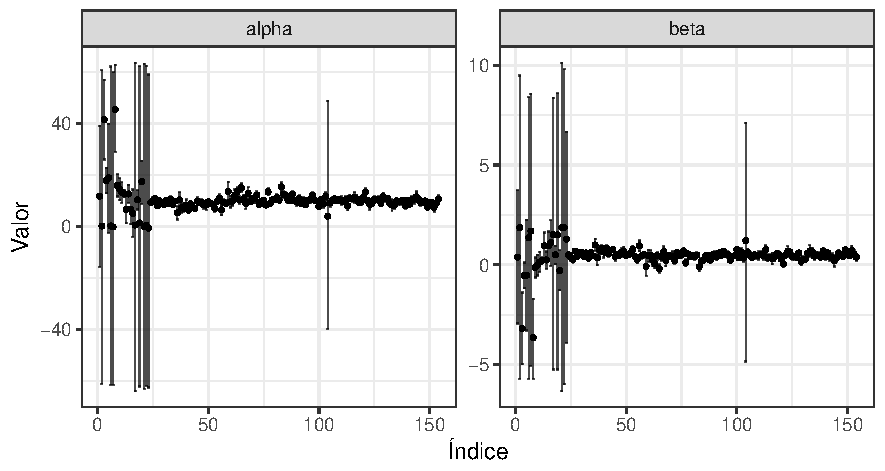
\includegraphics[width=0.7\textwidth]{images/no_pooling_param_values.pdf}
    \caption{Valor e intervalos de probabilidad de parámetros de modelo de unidades independientes}
    \label{fig:no_pooling_param_values}
\end{figure}

\begin{figure}[H]
    \centering
    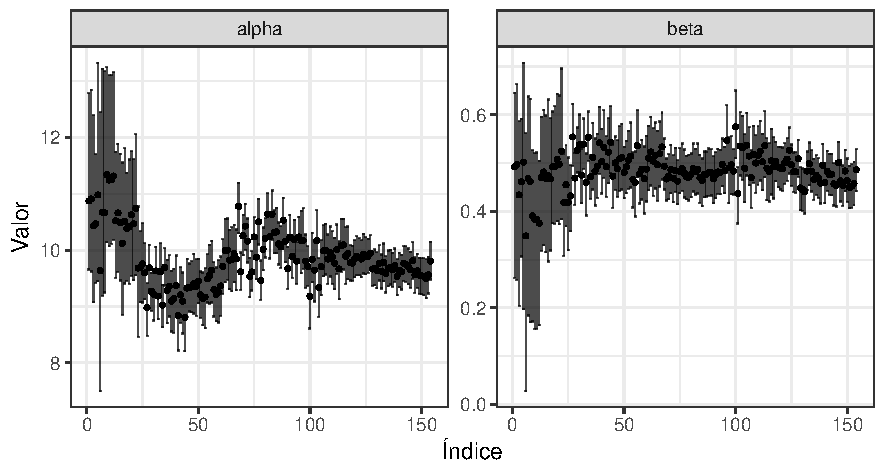
\includegraphics[width=0.7\textwidth]{images/three_levels_param_values.pdf}
    \caption{Valor e intervalos de probabilidad de parámetros de modelo multinivel}
    \label{fig:three_levels_param_values}
\end{figure}

Para observar el efecto de las diferencias en los parámetros, en las figuras \ref{fig:no_pooling_obs_vs_pred_train_by_neighborhood_zip_regression_lines} y \ref{fig:three_levels_obs_vs_pred_train_by_neighborhood_zip_regression_lines} se muestran las pendientes de regresión de código postal de cada modelo. Cada figura tiene muchas subgráficas, cada una representando un vecindario. Dentro de cada subgráfica se muestran los puntos de las ventas y además las líneas de regresión ajustadas a cada código postal dentro de cada vecindario. Se puede ver que en el modelo de unidades independientes cambian mucho las líneas, sobre todo en los vecindarios en los que hay pocos datos, llegando a haber líneas con pendientes negativas, lo cual no tiene mucho sentido dado el contexto del problema. El modelo nivel muestra pendientes más estables, y sobre todo, en los vecindarios y códigos postales, se mantiene siempre la pendiente positiva.

\begin{figure}[H]
    \centering
    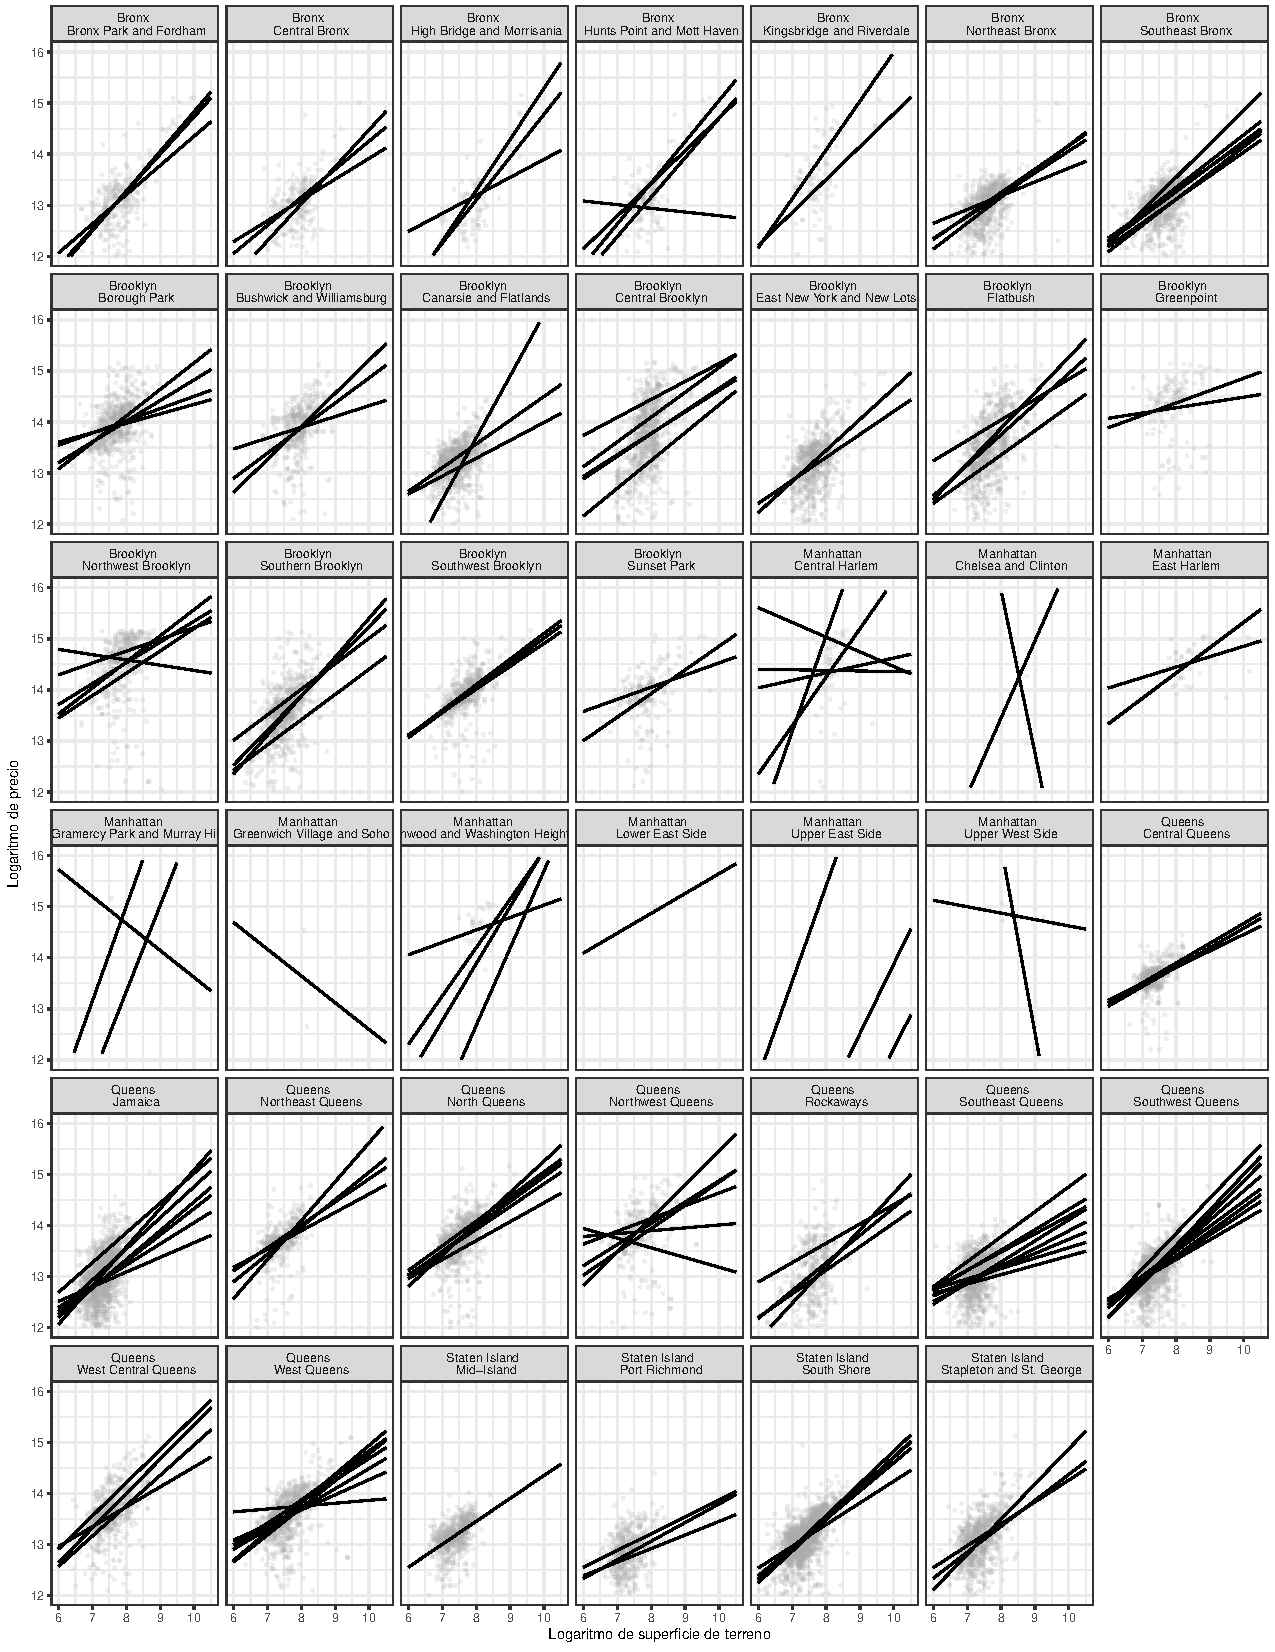
\includegraphics[width=\textwidth]{images/no_pooling_obs_vs_pred_train_by_neighborhood_zip_regression_lines.pdf}
    \caption{Modelo de unidades independientes: Diagramas de dispersión de logaritmo de superficie de terreno contra logaritmo del precio, separados por vecindario. Dentro de cada gráfica de vecindario, se muestran las líneas de regresión de cada código postal.}
    \label{fig:no_pooling_obs_vs_pred_train_by_neighborhood_zip_regression_lines}
\end{figure}

\begin{figure}[H]
    \centering
    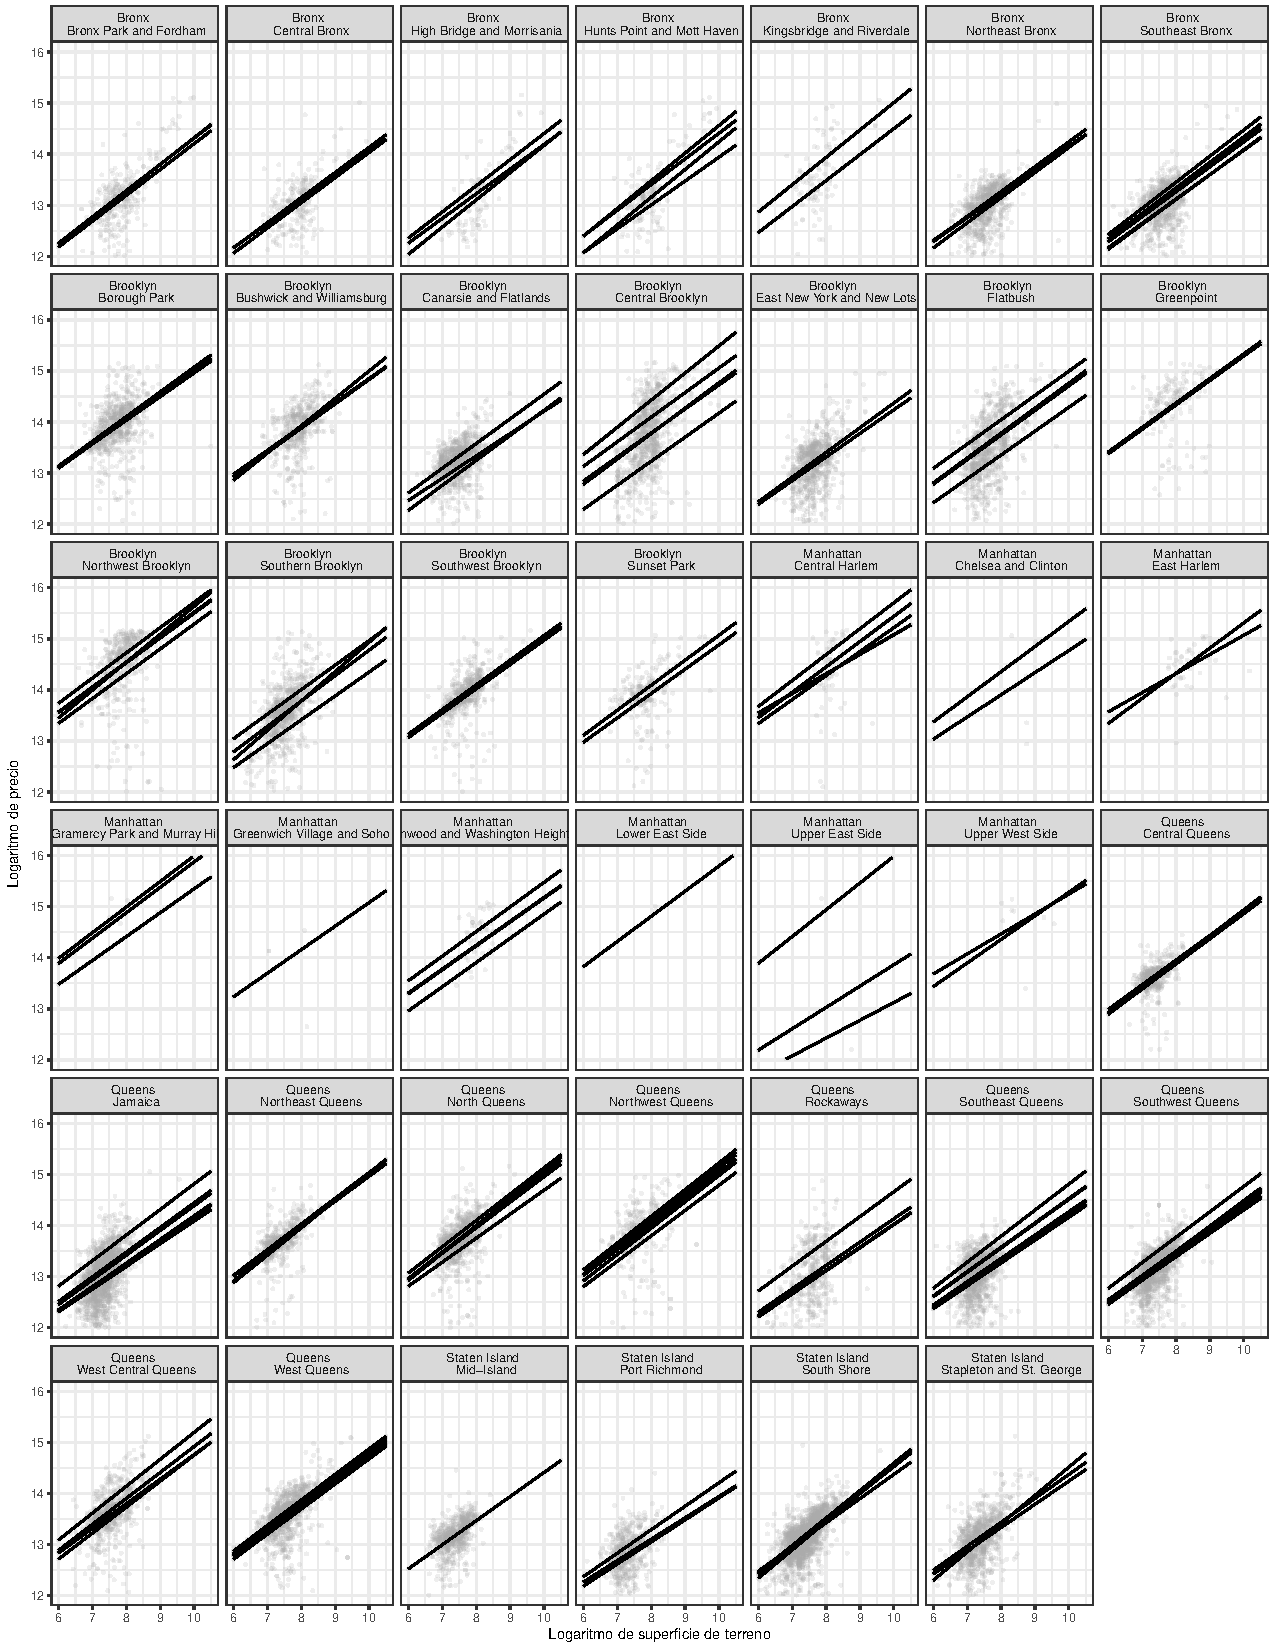
\includegraphics[width=\textwidth]{images/three_levels_obs_vs_pred_train_by_neighborhood_zip_regression_lines.pdf}
    \caption{Modelo multinivel: Diagramas de dispersión de logaritmo de superficie de terreno contra logaritmo del precio, separados por vecindario. Dentro de cada gráfica de vecindario, se muestran las líneas de regresión de cada código postal.}
    \label{fig:three_levels_obs_vs_pred_train_by_neighborhood_zip_regression_lines}
\end{figure}


Para medir el desempeño de los distintos modelos, se pueden usar distintas medidas. En este trabajo, se utilizan tres: el DIC (\textit{Deviance Information Criterion}), la raíz del error cuadrático medio (RMSE) y el error medio absoluto (MAE). Dada su definición, para las tres medidas, es preferible tener un menor valor. Sean $y_i$ los valores observados y $\hat{y_i}$ las estimaciones puntuales para cada $i \in \left\{ 1, \hdots, n \right\}$, donde $n$ es el número total de observaciones. Las cantidades antes mencionadas están definidas como

\[
	\mathrm{RMSE} = \sqrt{ \frac{1}{n} \sum_{i = 1}^n \left( y_i - \hat{y_i} \right)^2 }
\]

\[
	\mathrm{MAE} = \frac{1}{n} \sum_{i = 1}^n \left| y_i - \hat{y_i} \right|
\]

\[
	\mathrm{DIC} = -2 \log{p(y | \theta)} + 2 \log{h(y)},
\]

donde $p(y | \theta)$ es la función de verosimilitud y $h(y)$ es una función de estandarización de los datos.

En la tabla \ref{tab:dic_rmse_mae} se muestran los valores de estas medidas para cada uno de los modelos. El modelo de unidades iguales es claramente inferior, pues los valores son mucho mayores. Entre el modelo de unidades independientes y el multinivel hay competencia, pues el primero tiene mayor DIC pero menores MAE y RMSE. Sin embargo, las diferencias en MAE y RMSE no son muy grandes; y además, viendo los resultados anteriores, el modelo multinivel es más robusto que el de unidades independientes.

\begin{table}[]
	\centering
	\caption{Valores de DIC, RMSE y MAE de cada modelo.}
	\label{tab:dic_rmse_mae}
	\begin{tabular}{|l|c|c|c|c|c|}
	\hline
	                        &           & \multicolumn{2}{c|}{Entrenamiento} & \multicolumn{2}{c|}{Prueba} \\ \hline
	                        & DIC       & MAE              & RMSE            & MAE          & RMSE         \\ \hline
	Unidades iguales        & 630,996   & 287,374          & 461,166         & 283,847      & 446,443      \\ \hline
	Unidades independientes & 7,239,403 & 188,123          & 315,006         & 190,248      & 324,864      \\ \hline
	Multinivel              & 16,716    & 191,383          & 324,493         & 192,564      & 335,204      \\ \hline
	\end{tabular}
\end{table}

% > readRDS("../out/models/model_comp_pooling.rds")$BUGSoutput$DIC
% [1] 630996.6
% > readRDS("../out/models/model_no_pooling.rds")$BUGSoutput$DIC
% [1] 7239403
% > readRDS("../out/models/model_three_levels.rds")$BUGSoutput$DIC
% [1] 16716.46

% > (mae_train_comp_pooling <- mean(abs(preds_comp_pooling$res)))
% [1] 287374.6
% > (mae_test_comp_pooling <- mean(abs(preds_test_comp_pooling$res)))
% [1] 283847
% > (mae_train_no_pooling <- mean(abs(preds_no_pooling$res)))
% [1] 188123.9
% > (mae_test_no_pooling <- mean(abs(preds_test_no_pooling$res)))
% [1] 190248.7
% > (mae_train_three_levels <- mean(abs(preds_three_levels$res)))
% [1] 191383.7
% > (mae_test_three_levels <- mean(abs(preds_test_three_levels$res)))
% [1] 192564

% > (rmse_train_comp_pooling <- sqrt(mean(preds_comp_pooling$res^2)))
% [1] 461166.2
% > (rmse_test_comp_pooling <- sqrt(mean(preds_test_comp_pooling$res^2)))
% [1] 446443.7
% > # RMSEs
% > (rmse_train_no_pooling <- sqrt(mean(preds_no_pooling$res^2)))
% [1] 315006.2
% > (rmse_test_no_pooling <- sqrt(mean(preds_test_no_pooling$res^2)))
% [1] 324864.2
% > # RMSEs
% > (rmse_train_three_levels <- sqrt(mean(preds_three_levels$res^2)))
% [1] 324493.5
% > (rmse_test_three_levels <- sqrt(mean(preds_test_three_levels$res^2)))
% [1] 335204.5



% Gráficas del diagnóstico de Gelman para convergencia
% Comparar tamaño de muestra efectivo vs obtenido
% https://cran.r-project.org/web/packages/bayesplot/vignettes/visual-mcmc-diagnostics.html

% Probar con distintas priors y ver si resultados son los mismos

% Comparar coeficientes y promedios en distintos boroughs, vecindarios y zip codes
% Ver RMSE por borough y vecindario para cada modelo

% Mapa con valores de predicción junto con su correspondiente incertidumbre (la mitad de la longitud del intervalo de 95% de credibilidad)
% Modelo con dist T: http://doingbayesiandataanalysis.blogspot.mx/2013/06/bayesian-robust-regression-for-anscombe.html

% Comparar modelo final con modelo de interceptos distintos por zip sin jerearquía
% Comparar vs modelo nulo

% Analizar algunos outliers del modelo

%!TEX root = ../GLM_Becerra_Lopez.tex

\section{Conclusiones}
\label{sec:conclusiones}

Los tres modelos presentados anteriormente son soluciones a un mismo problema: predecir el precio de una casa en venta. El modelo de unidades iguales no considera la variabilidad de los precios dependiendo en la zona geográfica, lo que lo hace un modelo poco creíble desde su definición. El modelo de unidades independientes incorpora esta variabilidad pero no la capta en su totalidad, y aunque en algunas métricas de evaluación de ajuste salga mejor que los demás modelos, algunos de los resultados arrojados por el modelo no son lógicos. Finalmente, el modelo multinivel también incorpora la variabilidad de los precios pero a distintos niveles geográficos por lo es un modelo más robusto. Otra característica importante es que a diferencia de los otros modelos, el modelo multinivel utiliza toda la información disponible. Por lo que se concluye que el modelo multinivel es el mejor modelo para responder al problema planteado.

Es importante mencionar que aún cuando un modelo presenta mejores métricas de ajuste, no necesariamente es el que tiene mejor interpretabilidad, por lo que en la práctica estadística es recomendable comparar los resultados de un modelo contra la realidad. También creemos que las métricas de ajuste pueden mejorar con más covariables que describan las casas, por ejemplo, número de cuartos, número de baños, estado de la casa, etc. Sin embargo, en este ejercicio estas variables no estaban disponibles.

Asimismo, en este trabajo también se puede observar otra de las aplicaciones de los modelos de regresión: estimación de datos faltantes. Pues mediante el modelo multinivel se realizó una estimación de cual sería el precio de venta de un pie cudrado en códigos postales que no registrarón ventas.



\printbibliography
\nocite{*}

\newpage

%!TEX root = ../GLM_Becerra_Lopez.tex

\section*{Apéndice: convergencia de cadenas}
\label{sec:appendix}


\subsection*{Modelo de unidades iguales}

\begin{figure}[H]
    \centering
    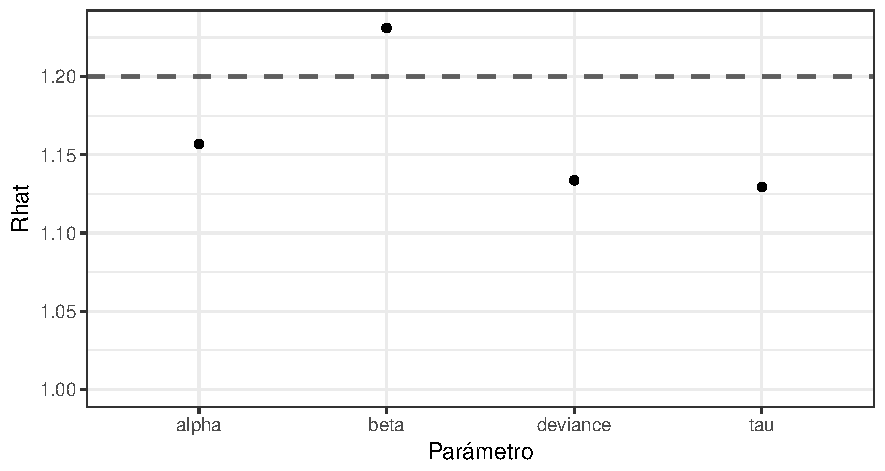
\includegraphics[width=0.9\textwidth]{images/comp_pooling_r_statistic_params.pdf}
    \caption{Estadística de convergencia $\hat{R}$ de Gelman y Rubin para cada parámetro del modelo de unidades iguales}
    \label{fig:comp_pooling_r_statistic_params}
\end{figure}

\begin{figure}[H]
    \centering
    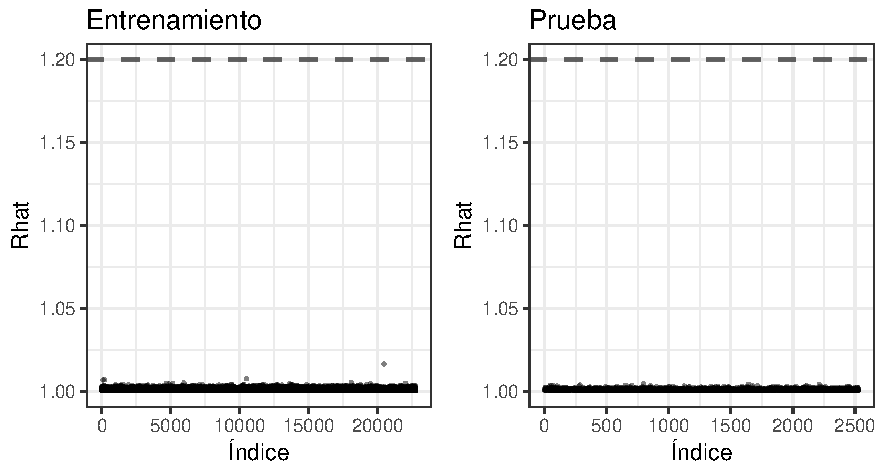
\includegraphics[width=0.9\textwidth]{images/comp_pooling_r_statistic_yf.pdf}
    \caption{Estadística de convergencia $\hat{R}$ de Gelman y Rubin para estimaciones de la variable respuesta del modelo de unidades iguales}
    \label{fig:comp_pooling_r_statistic_yf}
\end{figure}

\begin{figure}[H]
    \centering
    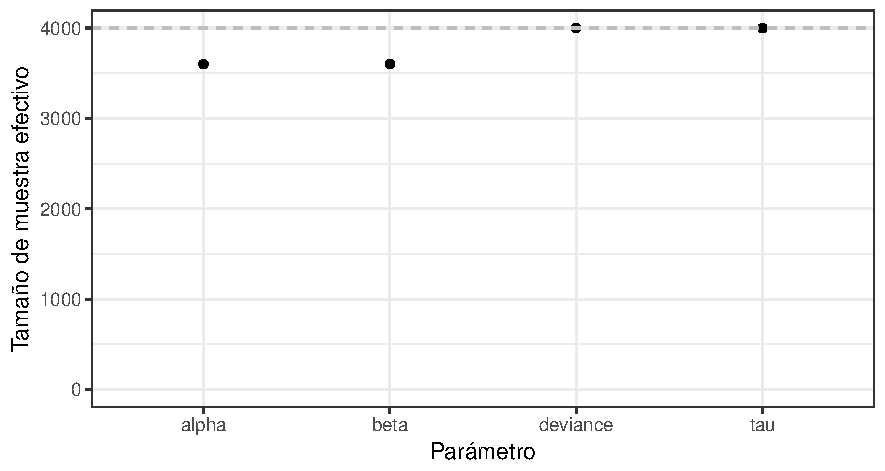
\includegraphics[width=0.9\textwidth]{images/comp_pooling_n_eff_params.pdf}
    \caption{Tamaño de muestra efectivo para cada parámetro del modelo de unidades iguales}
    \label{fig:comp_pooling_n_eff_params}
\end{figure}

\begin{figure}[H]
    \centering
    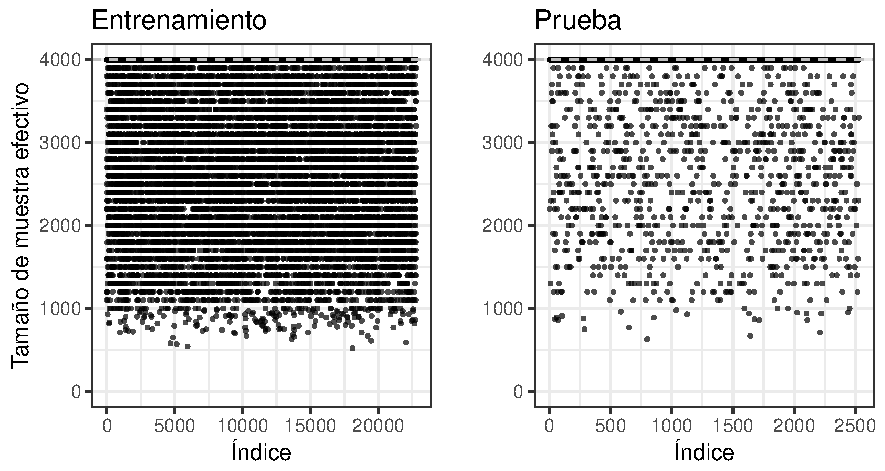
\includegraphics[width=0.9\textwidth]{images/comp_pooling_n_eff_yf.pdf}
    \caption{Tamaño de muestra efectivo para cada estimación de la variable respuesta del modelo de unidades iguales}
    \label{fig:comp_pooling_n_eff_yf}
\end{figure}



\subsection*{Modelo de unidades independientes}

\begin{figure}[H]
    \centering
    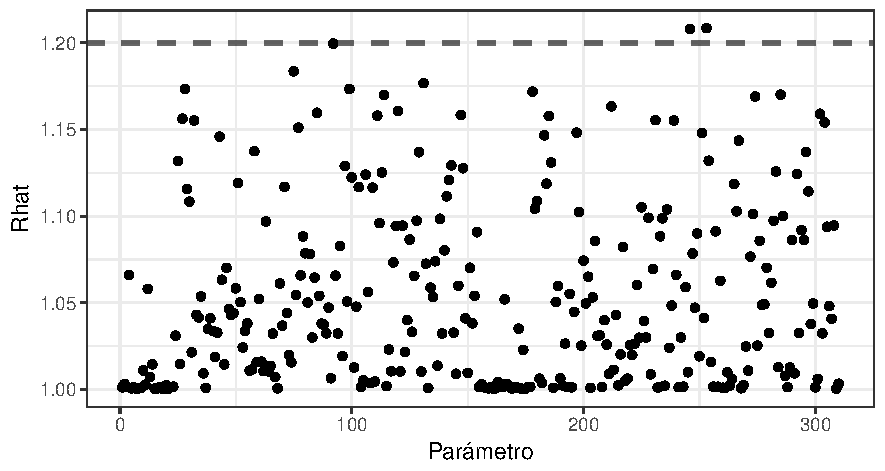
\includegraphics[width=0.9\textwidth]{images/no_pooling_r_statistic_params.pdf}
    \caption{Estadística de convergencia $\hat{R}$ de Gelman y Rubin para cada parámetro del modelo de unidades independientes}
    \label{fig:no_pooling_r_statistic_params}
\end{figure}

\begin{figure}[H]
    \centering
    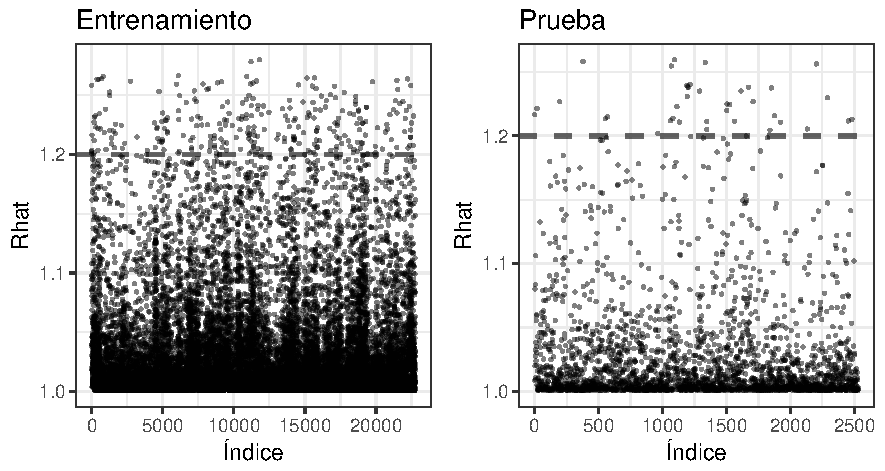
\includegraphics[width=0.9\textwidth]{images/no_pooling_r_statistic_yf.pdf}
    \caption{Estadística de convergencia $\hat{R}$ de Gelman y Rubin para estimaciones de la variable respuesta del modelo de unidades independientes}
    \label{fig:no_pooling_r_statistic_yf}
\end{figure}

\begin{figure}[H]
    \centering
    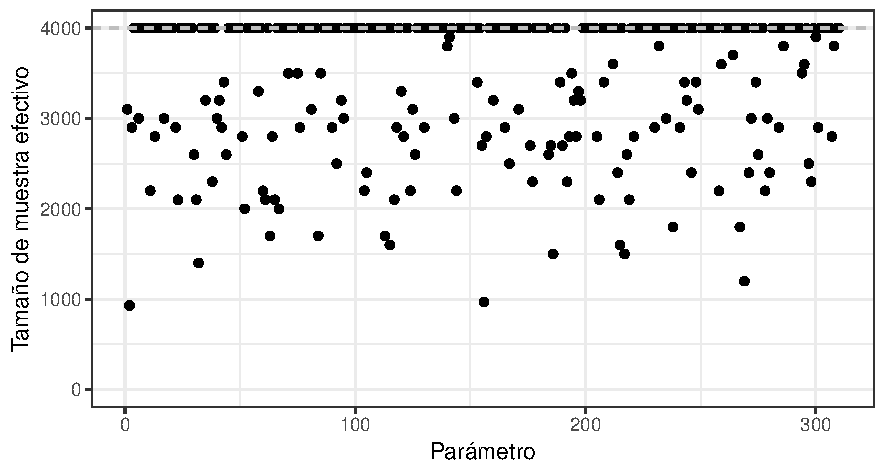
\includegraphics[width=0.9\textwidth]{images/no_pooling_n_eff_params.pdf}
    \caption{Tamaño de muestra efectivo para cada parámetro del modelo de unidades independientes}
    \label{fig:no_pooling_n_eff_params}
\end{figure}

\begin{figure}[H]
    \centering
    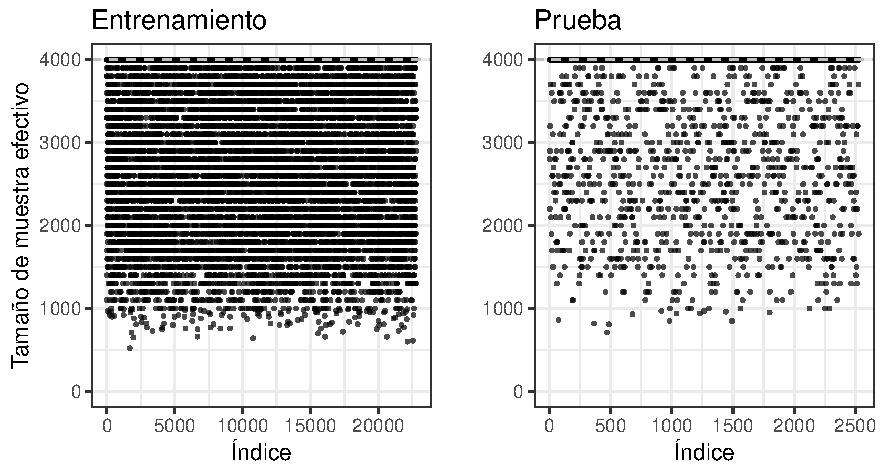
\includegraphics[width=0.9\textwidth]{images/no_pooling_n_eff_yf.pdf}
    \caption{Tamaño de muestra efectivo para cada estimación de la variable respuesta del modelo de unidades independientes}
    \label{fig:no_pooling_n_eff_yf}
\end{figure}




\subsection*{Modelo multinivel}

\begin{figure}[H]
    \centering
    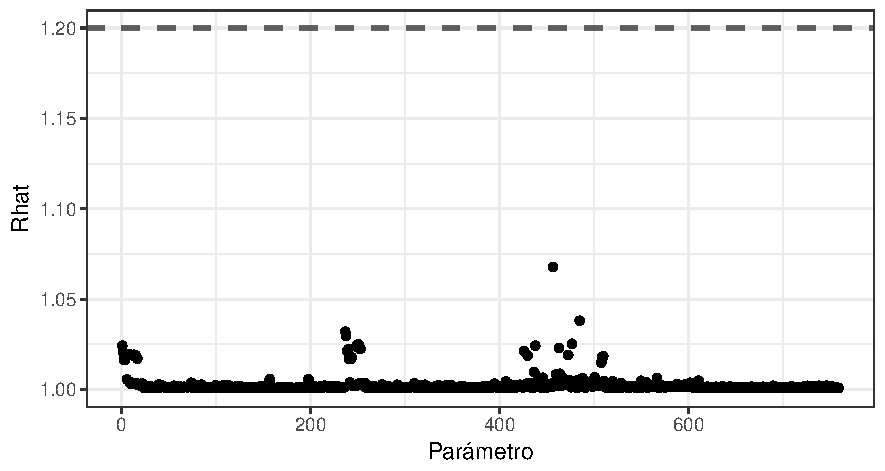
\includegraphics[width=0.9\textwidth]{images/three_levels_r_statistic_params.pdf}
    \caption{Estadística de convergencia $\hat{R}$ de Gelman y Rubin para cada parámetro del modelo multinivel}
    \label{fig:three_levels_r_statistic_params}
\end{figure}

\begin{figure}[H]
    \centering
    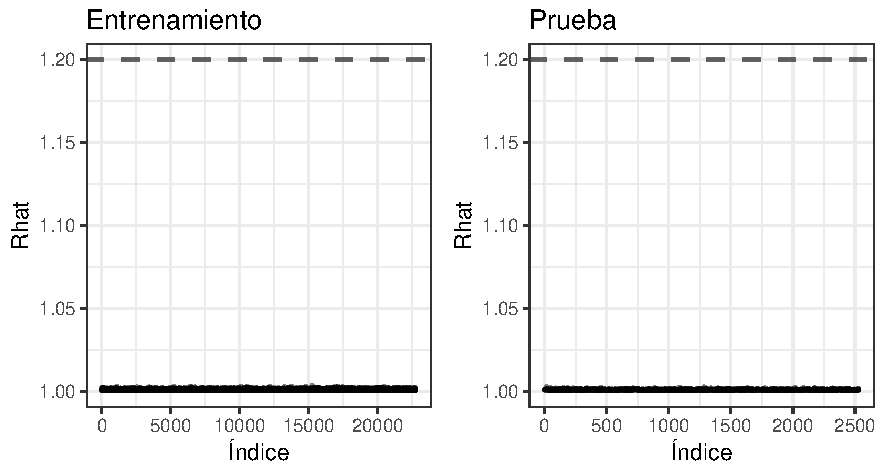
\includegraphics[width=0.9\textwidth]{images/three_levels_r_statistic_yf.pdf}
    \caption{Estadística de convergencia $\hat{R}$ de Gelman y Rubin para estimaciones de la variable respuesta del modelo multinivel}
    \label{fig:three_levels_r_statistic_yf}
\end{figure}

\begin{figure}[H]
    \centering
    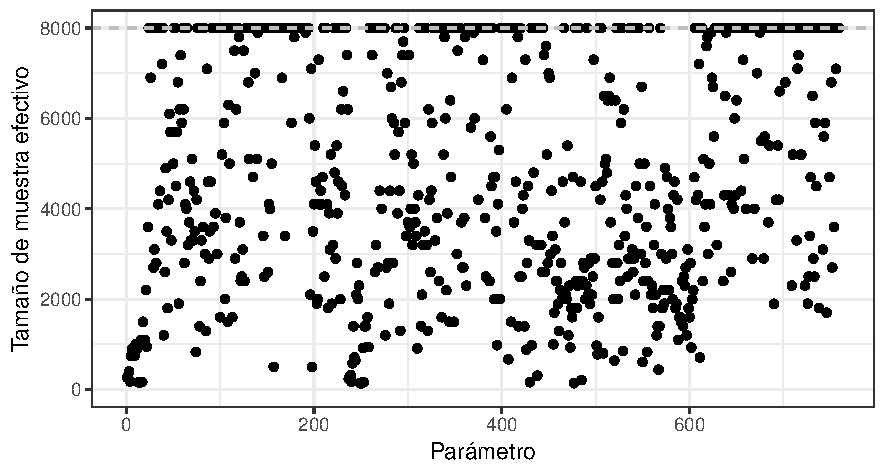
\includegraphics[width=0.9\textwidth]{images/three_levels_n_eff_params.pdf}
    \caption{Tamaño de muestra efectivo para cada parámetro del modelo multinivel}
    \label{fig:three_levels_n_eff_params}
\end{figure}

\begin{figure}[H]
    \centering
    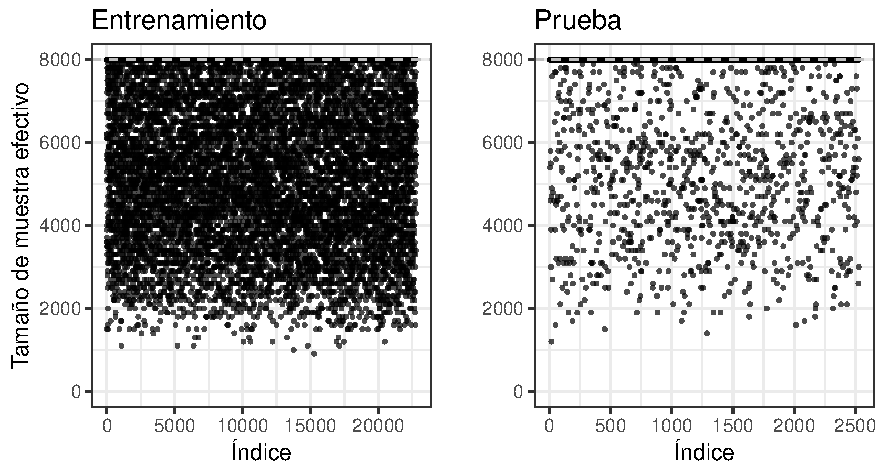
\includegraphics[width=0.9\textwidth]{images/three_levels_n_eff_yf.pdf}
    \caption{Tamaño de muestra efectivo para cada estimación de la variable respuesta del modelo multinivel}
    \label{fig:three_levels_n_eff_yf}
\end{figure}



\end{document}
